%16章 
\chapter{进阶三角比}
\label{ch:Further Trig}

\section*{学习目标}
\begin{todolist}
 \item 理解正割,余割和余切的定义
 \item 从余弦,正弦,正切函数图像推导正割,余割和余切的函数图像
 \item 掌握并利用三角比其他恒等式
 \item 掌握并利用正弦,余弦,正切的和差角公式
 \item 掌握并利用二倍角公式
 \item 掌握并利用辅助角公式
\end{todolist}
\clearpage

\section{正割,余割与余切}
之前定义了正弦,余弦和正切比。现在将要拓展至另外三个比率。其实难度不大。
\begin{figure}[H]
\centering
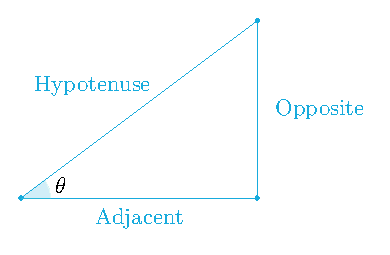
\includegraphics[width=0.5\textwidth]{sec}
\caption{继续沿用锐角三角形中的对邻斜关系}
\end{figure}

\subsection*{正割}
于是\gls{sec}被定义为:
\[
	\sec \theta=\frac{\text{Hypotenuse}}{\text{Adjacent}}=\frac{1}{\cos \theta}
\]

\subsection*{余割}
\gls{csc}被定义为:
\[
	\csc \theta=\frac{\text{Hypotenuse}}{\text{Opposite}}=\frac{1}{\sin \theta}
\]

\subsection*{余切}
\gls{cot}被定义为:
\[
	\cot \theta=\frac{\text{Adjacent}}{\text{Opposite}}=\frac{1}{\tan \theta}
\]

因此这三个新的三角比的研究并没有比$\sin$,$\cos$,$\tan$更复杂。

\subsection*{函数图像的关系} %有点太长了
因此绘制$6$个三角函数的图像为:
\begin{figure}[H]
\centering
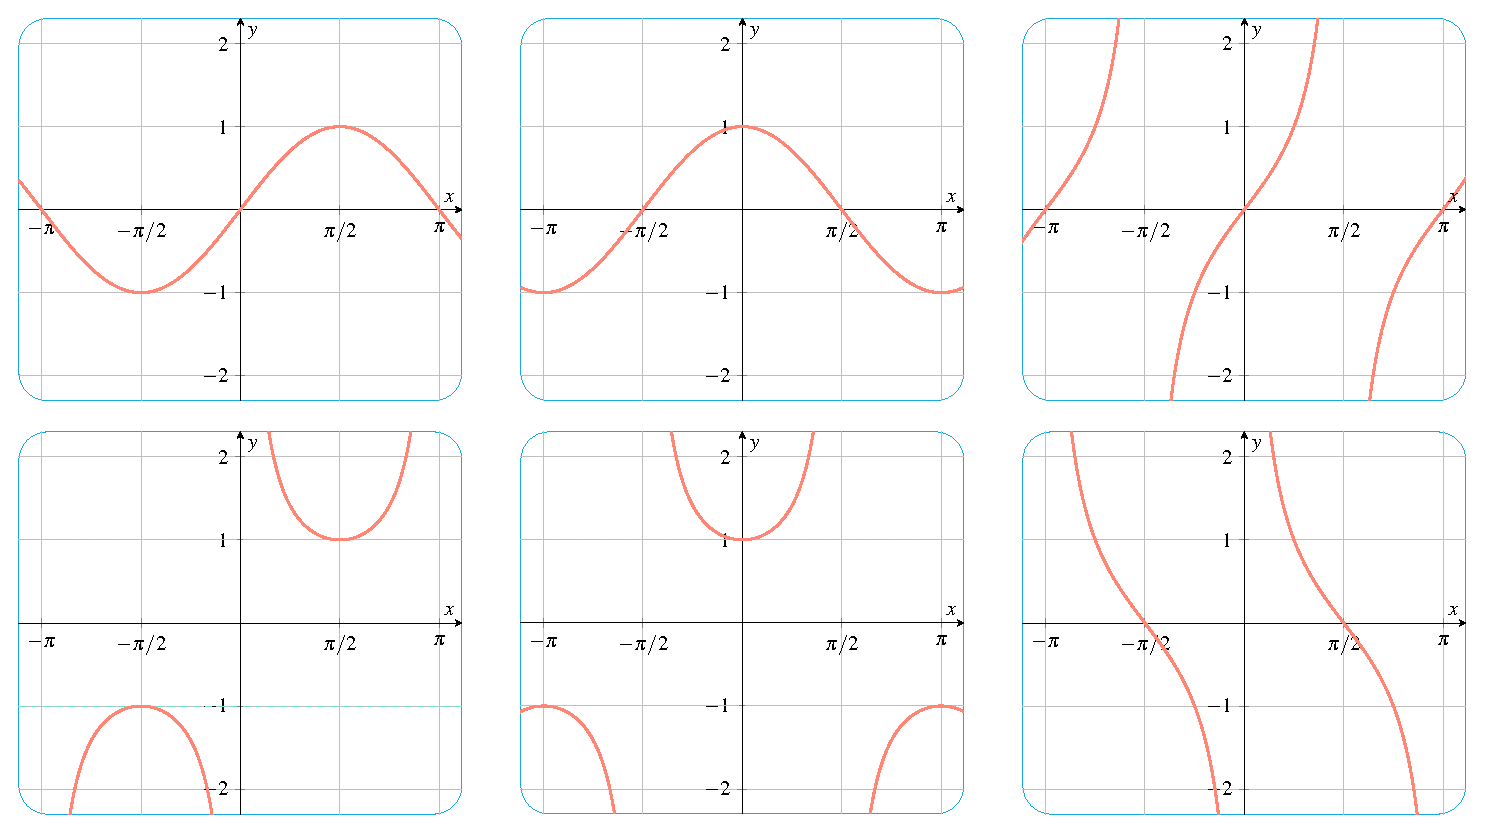
\includegraphics[width=\textwidth]{sixtrig}
\caption{常见的三角函数}
\end{figure}

\begin{TaskBox}
 明确这六张函数图像所对应的表达式:$y=\sin x$, $y=\cos x$,$y=\tan x$, $y=\sec x$, $y=\cot x$,$y=\cot x$。
\end{TaskBox}
\clearpage

\section{三角恒等式}
\label{sec:Trig Identity}
从三角函数的定义可以推导推导出很多的恒等式,归纳概括起来可以用这样的一张表进行描述:
\begin{figure}[H]
\centering
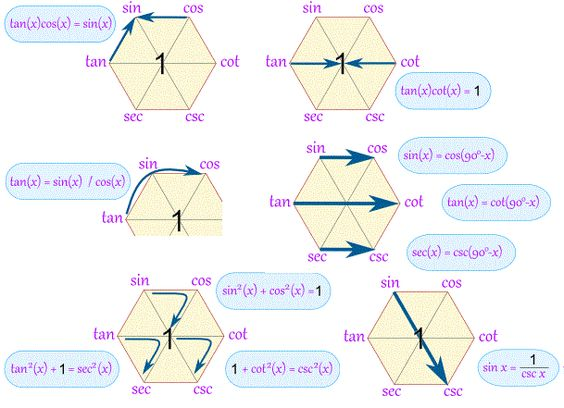
\includegraphics[width=\textwidth]{trighexa}
\caption{三角恒等式的六边形}
\end{figure}
这些解释如下:

\subsection*{倒数关系}
\begin{minipage}{0.7\linewidth}
在任意的斜对角线的上的三角比互为相反数:
\begin{align*}
	\cos x \cdot \sec x &= 1\\
	\sin x \cdot \csc x &= 1\\
	\tan x \cdot \cot x &= 1
\end{align*}
\end{minipage}
\hfill
\begin{minipage}{0.25\linewidth} %这里过大了
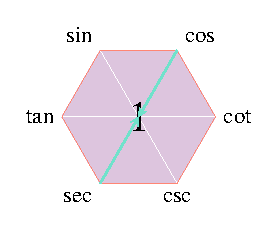
\includegraphics[width=\textwidth]{reci}
\end{minipage}

\subsection*{除法关系}
\begin{minipage}{0.7\linewidth}
如右图所示,在任意相连的箭头当中,第一个三角比总是等于另外两个相除:
\begin{align*}
	\tan x &= \frac{\sin x}{\cos x}\\
	\cot x &=\frac{\csc x}{\sec x}
\end{align*}
\end{minipage}
\hfill
\begin{minipage}{0.3\linewidth}
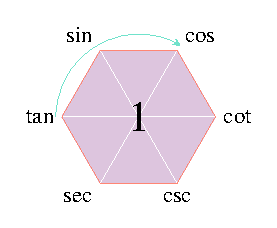
\includegraphics[width=\textwidth]{ratio}
\end{minipage}

\begin{TaskBox}
完成剩余的$4$个比例
\end{TaskBox}

\subsection*{互余相等}
\begin{minipage}{0.7\linewidth}
从左往右方向上,如果两个角的互余,则三角比相等。
\begin{align*}
	\sin x &= \cos \left(\frac{\pi}{2}-x\right)\\
	\tan x &= \cot \left(\frac{\pi}{2}-x\right)\\
	\sec x &= \csc \left(\frac{\pi}{2}-x\right)
\end{align*}
\end{minipage}
\hfill
\begin{minipage}{0.3\linewidth}
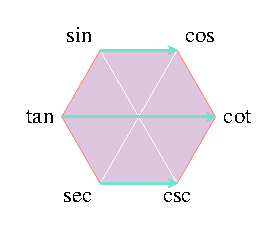
\includegraphics[width=\textwidth]{complementary}
\end{minipage}

\subsection*{平方和差与$1$的关系}
\begin{minipage}{0.7\linewidth}
按照图中绿色箭头的方式顶点上的两个平方等同于下方的平方:
\begin{align*}
	\sin^2 x+\cos^2 &=1^2 \\
	\tan^2 x+1^2 &=\sec^2 x \\
	1^2+ \cot^2 x &=\csc^2 x
\end{align*}
\end{minipage}
\hfill
\begin{minipage}{0.3\linewidth}
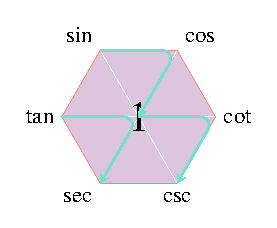
\includegraphics[width=\textwidth]{squaresum}
\end{minipage}
\clearpage

\section{三角比当中的公式}
这些公式都是考试中重点,但是不做推导,仅需记忆和利用。

\subsection*{和差角公式}
\begin{align*}
\sin \left( \alpha + \beta\right) &= \sin\alpha \cos\beta
+\cos \alpha \sin \beta\\
\sin \left( \alpha - \beta\right) &= \sin\alpha \cos\beta
-\cos \alpha \sin \beta\\
\cos \left( \alpha + \beta\right) &= \cos\alpha \cos\beta
-\sin \alpha \sin \beta\\
\cos \left( \alpha - \beta\right) &= \cos\alpha \cos\beta
+\sin \alpha \sin \beta\\
\tan \left( \alpha + \beta\right) &= \frac{\tan \alpha +\tan \beta}{1-\tan \alpha \tan \beta}\\
\tan \left( \alpha - \beta\right) &= \frac{\tan \alpha -\tan \beta}{1+\tan \alpha \tan \beta}
\end{align*}
可以查看\href{https://www.bilibili.com/video/BV1kN411Q7aP}{三角恒等变换的可视化}了解证明过程

\subsection*{二倍角公式}
\label{subsec:Double Angle Formula}
把和角公式当中替换为两个相等的角就得到了二倍角公式。
\begin{align*}
 \sin 2\alpha &= 2\sin \alpha \cos \alpha\\
 \cos 2\alpha &= \cos^2 \alpha -\sin^2 \alpha\\
 			  &=2\cos^2 \alpha-1\\
 			  &=1 - 2\sin^2 \alpha\\
 \tan 2\alpha &= \frac{2\tan \alpha}{1-\tan^2 \alpha}
\end{align*}


\begin{ExampleBox}
Prove the identity $\tan (45\si{\degree}+x)+\tan (45\si{\degree} -x)\equiv 2 \sec 2x$\\
\makebox{}\hfill Adapted From 2017 winter qp31 Q4
\tcblower
此题解决可以有多种做法,下方展示直接利用$\tan$的和差角公式进行
\begin{align*}
 LHS &= \frac{\tan 45^{\circ}+\tan x}{1-\tan 45^{\circ}\cdot \tan x}+\frac{\tan 45^{\circ}- \tan x}{1+\tan 45^{\circ}\cdot \tan x}\\
     &= \frac{1+\tan x}{1-\tan x}+\frac{1-\tan x}{1+\tan x}\\
     &= \frac{(1+\tan x)^2+(1-\tan x)^2}{1-\tan^2 x}\\
     &=\frac{2+2\tan^2 x}{1-\tan^2 x}\\
     &=2\cdot \frac{1+\tan^2 x}{1-\tan^2 x} \quad {\text{同时乘以$\cos^2 x$}}\\ 
     &=2\cdot \frac{\cos^2 x+\sin^2 x}{\cos^2 x-\sin^2 x}\\
     &=2 \cdot \frac{1}{\cos 2x} \quad \text{二倍角公式}\\
     &=2 \sec 2x\\
     &=RHS
\end{align*}
QED,证明完毕
\end{ExampleBox}


\subsection*{辅助角公式}
辅助角公式是正弦的和差的利用。是处理$a\sin\theta+b\cos\theta$的公式。
公式为:
\[
	a\sin\theta+b\cos\theta = R\cdot \sin(\theta+\phi)
\]
其中:
\begin{align*}
 R &= \sqrt{a^2+b^2}\\
 \phi &= \arctan \frac{b}{a}
\end{align*}

\begin{ExampleBox}
 证明的过程如下:
 \tcblower
 \begin{align*}
 a\sin\theta+b\cos\theta &= R\cdot \left( \frac{a}{R}\sin\theta + \frac{b}{R}\cos\theta \right)\\
 						&= R\cdot \left(\cos \phi \sin \theta +\sin \phi \cos \theta \right)\\
 						&=R\cdot \sin(\theta+\phi)
 \end{align*}
 $a$,$b$,$R$构成一个如下图的辅助三角形。$\phi$是$b$所对的角。
 \begin{figure}[H]
 \centering
 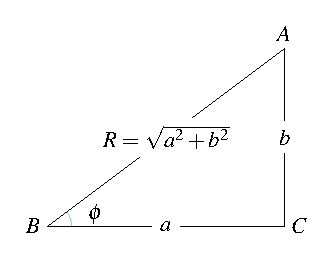
\includegraphics[width=0.8\textwidth]{auxitriangle}
 \caption{辅助三角形的确定}
 \end{figure}
 
\end{ExampleBox}


